% Created 2015-06-23 Tue 12:39
\documentclass[11pt]{article}
\usepackage[utf8]{inputenc}
\usepackage[T1]{fontenc}
\usepackage{fixltx2e}
\usepackage{graphicx}
\usepackage{longtable}
\usepackage{float}
\usepackage{wrapfig}
\usepackage{rotating}
\usepackage[normalem]{ulem}
\usepackage{amsmath}
\usepackage{textcomp}
\usepackage{marvosym}
\usepackage{wasysym}
\usepackage{amssymb}
\usepackage{hyperref}
\usepackage{graphicx}
\tolerance=1000
\author{Nate Chodosh}
\date{\today}
\title{MBR Tracking Algorithm}
\hypersetup{
  pdfkeywords={},
  pdfsubject={},
  pdfcreator={Emacs 24.3.1 (Org mode 8.2.10)}}
\begin{document}

\maketitle

\section{Algorithm}
\label{sec-1}

\subsection{Structure of a model}
\label{sec-1-1}

The main data type of the tracking algorithm is the
Model. The Model stores all of the relevant information for tracking
and exposing a MBR. The fundamental representation of a Model is its
contour, which consists of a set of points that make up the edge of
the structure. The Model implements tracking with a
series of vectors that store information about the model at every
frame. There are three main pieces of information to be calculated
at each frame: the object's center, orientation, and the contour
found in that frame.

\subsection{Filtering and finding contours}
\label{sec-1-2}

The process of extracting the contours from an image is used
multiple times throughout the tracking algorithm so I will describe
it first here.

The first step is to remove the blue channel from the image to
separate the structures from any light projected
on the stage. Next the image is converted grayscale and then to a binary image using
an adaptive threshold which causes any areas of rapid intensity
change to be set to 1 and every other area set to 0. This
effectively highlights the edges of the contour as well as any
other noise in the image. The light or "on" areas are then expanded
using an erode method to close any small gaps in the edges of the
structures. Then the find contours method is used to extract all of
the shapes present in the image. Finally the noise is filtered out by
only taking contours with an enclosed area in a specified range.

\begin{figure}[h!]
  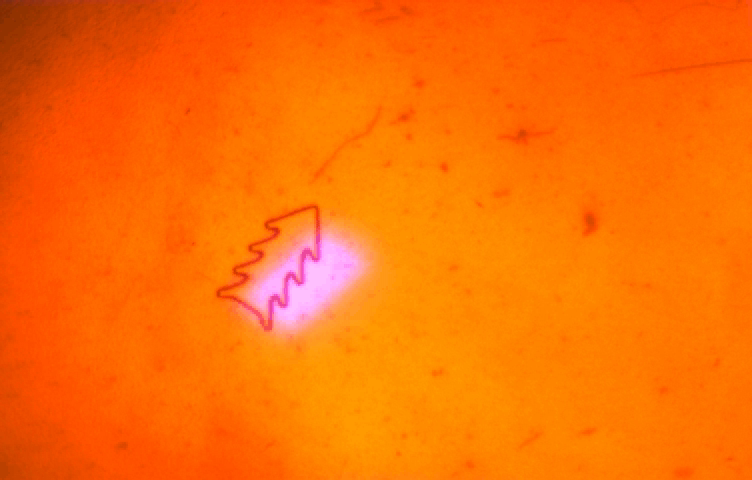
\includegraphics[width=0.5\textwidth]{original-0000}
  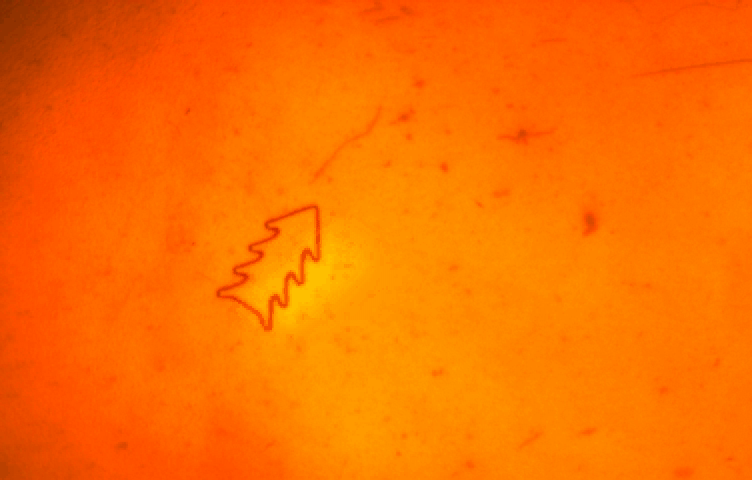
\includegraphics[width=0.5\textwidth]{no_blue-0000}
  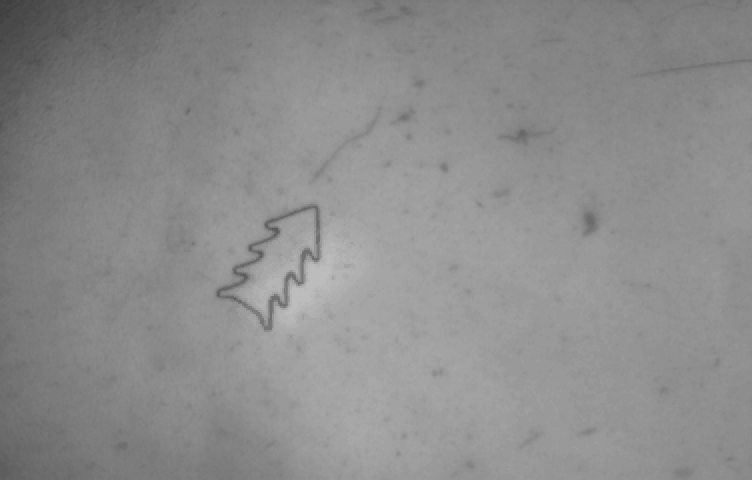
\includegraphics[width=0.5\textwidth]{grayscale-0000}
  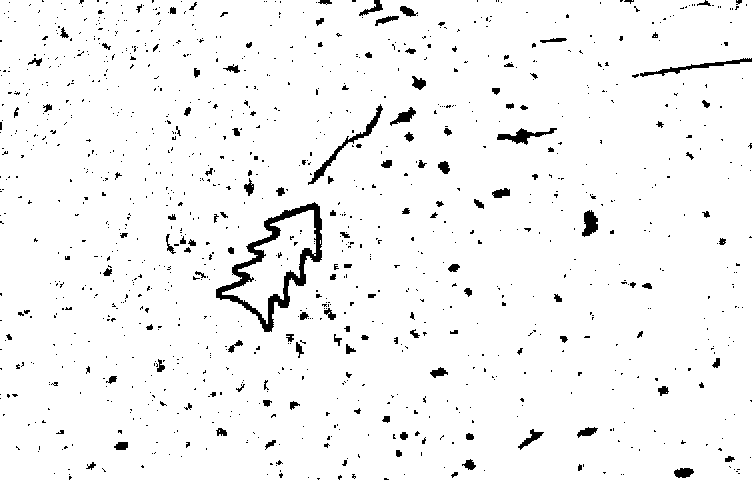
\includegraphics[width=0.5\textwidth]{adaptive_thresh-0000}
  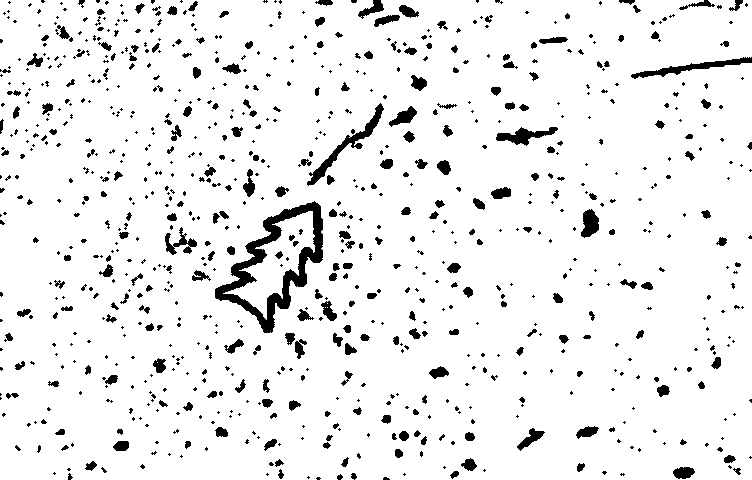
\includegraphics[width=0.5\textwidth]{eroded-0000}
  
\includegraphics[width=0.5\textwidth]{contours-0000}
  \caption{From left to right and top to bottom these images show each step of the contour
  finding algorithm.}
\end{figure}

\subsection{Warping}
\label{sec-1-3}

Before tracking the Models some calibration is in order to correct
for the distortion created by the projection method. To calibrate
the setup the user is asked to identify the position of 3 pairs of points as
they exist on both the stage and the DMD. These pairs are then used
to compute an affine transformation between the two planes. From
this point on any images to be projected are first run through that
transformation.

\subsection{Tracking}
\label{sec-1-4}

\subsubsection{Generating models}
\label{sec-1-4-1}

The first step in tracking is to find all of the potential
models. All potential contours are checked for an area inside
the given range and a Model object is created with the initial
information about the contour. The algorithm then begins to track
all of the potential models while the user selects which models
are of interest. Then the tracking is restarted using only those
models. The tracking needs to start before the user selects the
models since the algorithm relies on each model not moving too
much between frames.

\subsubsection{Updating models}
\label{sec-1-4-2}

The actual tracking itself is performed by capturing a frame and
using it to update all of the models from the previous frame. To
do this the following process is performed on each model in
turn. First a small region of interest around the previous
position of the model is identified and contours are extracted
from it using the normal method. Then these contours are searched
for the one whose area most closely matches the area of the
initial model. If the two areas are close enough the model is
considered to be 'found' in that frame. If the object is found the
contour is then used to determine the other two pieces of tracking
information, the center and the orientation. 

Calculating the center is done by simply computing the center of
mass of all of the contour points. Determining the orientation is
more difficult since the algorithm is designed to operate on
arbitrary contours which could have any amount of rotational
symmetry. To simplify this issue we compute a sort of polar
histogram of the contour called an orientation signal (Figure 2). The
histogram has 360 slots, one for each degree. Each slot contains
the average distance from the center to all points in the contour
that lie in that direction. In this form a rotation of the object
corresponds to a phase shift of this signal. Calculating the
phase shift that gives the minimum change in angle from the
previous frame then gives the new orientation provided the object
can't rotate fast enough in one frame to reach a point of symmetry
since in that case it would be impossible to determine the
orientation. Finally the information is added to the tracking
vectors of the model.

\begin{figure}[h!]
  \begin{center}
    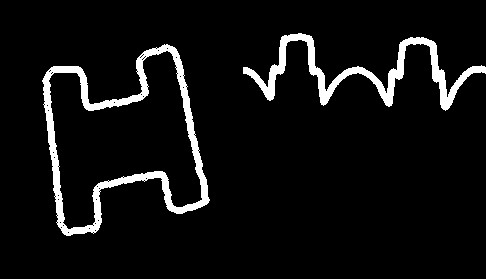
\includegraphics[width=0.6\textwidth]{rotation_signal-0000}    
  \end{center}

  \caption{A model and its rotation signal}
  \label{fig:rotation_signal}
\end{figure}
\subsection{Projecting}
\label{sec-1-5}

While the tracking occurs the user is presented with a visualization
of all the tracked models current state. Then the user can select
which model to expose at any time. There are two categories of
exposure to select from. Within each category the user can select
different types of exposure for each model which are then toggled on
off throughout the experiment. The first category is contour based. In
this type of exposure the entire contour of a microrobot is exposed
except for a specific region selected by the user. The second category
is not contour based. In this category the user selects which regions
of the robot to expose based only on the orientation of the robot
without any information about the specific shape of the contour. For
example the user may choose to expose a rectangle covering the top
half of a robot. Both types of exposure are shown in Figure 3

\begin{figure}[h!]
  \begin{center}
    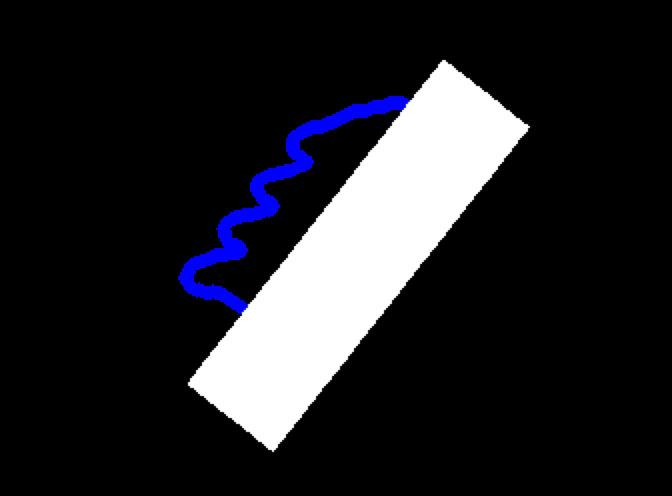
\includegraphics[width=0.4\textwidth]{exposure}    
    
\includegraphics[width=0.4\textwidth]{mask}    
  \end{center}

  \caption{Left: A non-contour based exposure, the contour is shown in blue but does not appear in the actual projection. Right: A contour based exposure that exposes the bottom half of the contour}
  \label{fig:rotation_signal}
\end{figure}

% Emacs 24.3.1 (Org mode 8.2.10)
\end{document}